\documentclass[12pt]{article}
\usepackage{amsmath}
\usepackage{jheppub}
\usepackage{marginnote,xparse,changepage,caption,graphicx,subcaption}

\newcommand{\IGNORE}[1]{}
\newcommand{\be}{\begin{equation}}
\newcommand{\ee}{\end{equation}}
\newcommand{\bea}{\begin{aligned}}
\newcommand{\eea}{\end{aligned}}
\newcommand{\F}[1]{F_{#1}}
\renewcommand{\P}[1]{P_{#1}}
\newcommand{\BF}[1]{\mathbf{F}_{#1}}
\newcommand{\BP}[1]{\mathbf{P}_{#1}}
\newcommand{\mb}[1]{\marginnote{\texttt{\small MB:\,#1}}}
\renewcommand{\ij}[1]{\marginnote{\texttt{\small IJ:\,#1}}}
\newcommand{\ibar}{{\overline{\emph\i}}}
\newcommand{\jbar}{{\overline{\emph\j}}}

\title{Boundary terms in the action for Causal Sets}
 \author[a]{Michel Buck}
 \author[a,b]{\!, Fay Dowker}
 \author[a]{\!, Ian Jubb\,}
 \author[c]{and Sumati Surya}
\affiliation[a]{Theoretical Physics Group, Blackett Laboratory, Imperial College, London, SW7 2AZ, U.K.}
\affiliation[b]{Institute for Quantum Computing, University of Waterloo, ON, N2L 2Y5, Canada}
\affiliation[c]{Raman Research Institute, CV Raman Ave, Sadashivanagar, Bangalore 560080, India}

\abstract{ 
We propose a family of formulae for the boundary term in the action of a causal set that is well-approximated by a continuum manifold with spacelike boundary. %The boundary term is proportional to the difference in the number of elements immediately to future and the number of elements immediately to the past of the surface. 
We show that in the continuum limit one recovers the Gibbons-Hawking-York boundary term in the mean.
}

\begin{document}

\maketitle

\section{Introduction}

%[MB1: USEFUL QUOTE FROM RAFAEL: In the quantum theory, however, these boundary terms are important. They are essential in order that the quantum mechanical amplitudes satisfy the correct composition law and in order that these amplitudes have the correct classical limit. In a number of examples [5] they give a contribution to the partition function which is important for the agreement with calculations based on straightforward thermodynamics. In this note we shall derive the boundary terms in the action for the Regge calculus]

In furthering causal set theory it is crucial that we understand the kinematics of the theory. The action of a given causal set (also causet) is a crucial piece of the kinematics that would be extremely useful to know and understand. Proposals for the action of a causal set are available \cite{Benincasa_Dowker:The_Scalar_Curvature_of_a_Causal_Set} and these hold analytically in some cases and numerically in many more.\mb{rephrase} One can show that the action of the causal set then agrees with the Einstein-Hilbert action of the spacetime in some continuum limit. How this limiting procedure is carried out will be described in more detail below.

It is well known that the Einstein-Hilbert action, $S_{EH}$, is not the full story in the continuum. In the presence of spacetime boundaries the gravitational action must include a boundary term $S_{GHY}$, the Gibbons-Hawking-York action, in order to yield a well-defined variational principle~\cite{Gibbons_Hawking_Boundary}. The contributions of this term play an essential role in particular in the quantum theory. For instance, in the calculation of the black hole entropy via the Euclidean path-integral, it is the boundary terms that produce the answer $A/4l_p^2$ necessary for the unification of black hole mechanics with thermodynamics. To give another example, in Regge calculus boundary terms are necessary in order that the quantum mechanical amplitudes satisfy the correct composition law and that they have the correct classical limit~\cite{hartlesorkin}.\mb{is this true?}

We define a \textit{causal set} (or \textit{causet}) as a locally finite partial order. This means it is a pair $ (\mathcal{C},\preceq)$ where $\mathcal{C}$ is the set of points and $\preceq$ is a partial order relation on $\mathcal{C}$ that has the following properties. It is (i) reflexive: $x\preceq x$, (ii) acyclic: $x\preceq y\preceq x \Rightarrow x=y$, and (iii) transitive: $x\preceq y\preceq z \Rightarrow x\preceq z$ for all points $x, y, z \in \mathcal{C}$. We define an inclusive order interval as the set $I (x,y)\equiv [ z\in\mathcal{C}|x\preceq z\preceq y]$ for any $x, y\in\mathcal{C}$. The \textit{locally finite} condition is simply that the cardinality of any order interval is finite, that is $|I (x,y)|<\infty$. This condition ensures we are dealing with a discrete structure, as all the other properties of the relation would apply to an order relation between points on a continuous Lorentzian manifold.

In order to say we have a causal set analogue for a continuous expression we need a well defined procedure for relating the discrete theory to the continuum. This procedure, or tool, is called a \textit{Poisson sprinkling}, or just a \textit{sprinkling}. It is a Poisson process which provides a way to generate a causet from a $d$-dimensional Lorentzian manifold $ (M,g)$ by selecting certain points in $M$ to be the elements of $\mathcal{C}$, with an order relation given by the causal order of the manifold. The number of points chosen in a region of spacetime volume, $V$, is a Poisson random variable. This means that the expected number of points in some region will be $\rho V$, where $\rho$ is the density of the sprinkling. The density is related to the discreteness scale, $l$, by $\rho=l^{-d}$ in $d$ spacetime dimensions. It is called a sprinkling as one can envisage the point selection process as a `sprinkling' of points into the manifold. If a causet, $\mathcal{C}$, can be generated with relatively high probability by a sprinkling into the manifold, $ (M,g)$, then we say that the manifold is a good approximation for the causal set, and that the causet can be \emph{faithfully embedded} in $M$.

\section{The Claims}

\subsection{Intuition and Relation to the Continuum}

Consider a sufficiently well-behaved $d$-dimensional spacetime $(M,g)$ which admits a \emph{spacelike partitioning} surface, $\Sigma$, defined as a spacelike closed compact surface in $M$, where the causal past and future sets, $M^\pm=J^\pm (\Sigma)$, of the surface then satisfy $M^+\cap M^-=\Sigma$. With this condition it follows that no points in $M^+\setminus\Sigma$ precede any points in $M^-\setminus\Sigma$. If there does exist a $p\in M^+\setminus\Sigma$ and a $q\in M^-\setminus\Sigma$ such that $p\preceq q$, then as $q\in J^-(\Sigma)$ we find that $p\in J^-(\Sigma)$, and hence it is in the set $M^-=J^-(\Sigma)$ by definition. The intersection, $M^+\cap M^-=\Sigma$, is now only true if $p\in\Sigma$ which it does not, and hence there cannot exist such a $p$.  We also have that $\partial M^\pm = \Sigma$. The Gibbons-Hawking-York boundary term for $M^\pm$ is in natural units given by
\be\label{eq:GHYBT_in_continuum}
{S}^{(d)}_{GHY}\left[M^\pm\right]= \mp \frac{1}{l_p^{d-2}}\int_{\Sigma} K d\Sigma
\ee
where $l_p$ is the rationalised Planck length for a general dimension, $l_p=(8\pi G)^{\frac{1}{d-2}}$ (where $G$ is the gravitational constant for a general dimension) and $K$ is the trace of the extrinsic curvature $K_{\mu\nu}=h_{\mu}^\rho h_\nu^\sigma \nabla_\rho n_\sigma$ of $\Sigma$ defined with future-pointing timelike unit normal covector $n_{\mu}=\partial_\mu S/\sqrt{g^{\mu\nu}\partial_\mu S\partial_\nu S}$. (We work with a mostly plus convention for the metric, in which this translates into a past-pointing normal vector $n^{\mu}$). Now observe that the integral in~\eqref{eq:GHYBT_in_continuum} can be thought of as the ``volume gradient'' across the surface $\Sigma$:
\be\label{eq:normal_deriv_boundary}
\int K d\Sigma = \frac{\partial}{\partial n}\int d\Sigma,
\ee
where the right hand side is the derivative of the area $\int d\Sigma$ as each point of $\Sigma$ is moved an equal distance along the unit normal vector, $n^{\mu}$ (corresponding to the rate of change of the surface volume \emph{backwards} in time, as $n^{\mu}$ is past-pointing).

Spacetime volume in the causal set is obtained simply by counting the number of elements, and hence the volume gradient intuitively corresponds to the difference in the number of ``immediate neighbours'' to the future and to the past of a hypersurface. In order to make this notion precise, we need to define the causal set analogue of a hypersurface, as well as an appropriate notion of ``closeness'' to it.

Given a causet that can be faithfully embedded in a manifold $M$ with a spacelike partitioning surface $\Sigma$, we obtain a natural partition of the causet into two parts $\mathcal{C}^+$ and $\mathcal{C}^-$, corresponding to the sets of elements that lie in $M^+=J^+(\Sigma)$ and $M^-=J^-(\Sigma)$. By virtue of $\Sigma$ being spacelike partitioning, the set $\mathcal C^-$ contains its own past, that is, any element in $\mathcal C$ that precedes at least one element in $\mathcal{C}^-$ is also in $\mathcal{C}^-$. Such a set is known as a \emph{past stem}. Similarly, $\mathcal C^+$ is a \emph{future stem} given an analogous definition. We propose more generally that for any causet $\mathcal C$, a \emph{spacelike partition} is a non-trivial partition that splits $\mathcal{C}$ into two parts, $\mathcal{C}^-$ and $\mathcal{C}^+=\mathcal{C}\setminus\mathcal{C}^-$ \IGNORE{($\mathcal{C}=\mathcal{C}^-\cup\mathcal{C}^+$)}, such that $\mathcal{C}^-$ is a past stem (or, equivalently, that $\mathcal{C}^+$ is a future stem and $\mathcal{C}^- = \mathcal{C}\setminus\mathcal{C}^+$). A sprinkling into a manifold with a surface such as $\Sigma$ will of course produce a causal set with spacelike partition, but we shall refer to a partition of a causal set satisfying the above definition as spacelike even when the causet is not obtained via a sprinkling into some manifold.

Determining rules for a partition to correspond to a timelike hypersurface in the continuum is extremely difficult and no satisfactory answer has been found yet. The situation for a null hypersurface is as follows. For any finite density sprinkling into a manifold (that admits a spacelike partitioning surface) with a null hypersurface, $\Sigma$, that null hypersurface will partition the causal set in such a way that agrees with our definition of a spacelike partition.\footnote{This fact means we should really refer to such a partition as ``non-timelike", but as we are dealing with spacelike hypersurfaces for most of this paper we shall continue to call such a partition spacelike}~The reason for this is that a causal set cannot distinguish between a null and spacelike hypersurface. To see why this is imagine a finite density sprinkling into a patch of $2$-dimensional Minkowski spacetime. Figure~\ref{fig:low_density_sprinkling_with_null_and_spacelike} shows how, given a null surface that partitions the causet into two parts, we can tilt the surface slightly so that it is now spacelike, while still preserving the partition. Figure~\ref{fig:high_density_sprinkling_with_null_and_spacelike} shows that even as we increase the density of the sprinkling we can tilt the surface by a smaller amount such that the partition remains unchanged. Hence, for any finite density sprinkling one can always find some slight deviation from a partitioning null hypersurface to one that is spacelike, while still preserving the partition. As the partition does not change we have no way of knowing whether the hypersurface is null or spacelike.

\begin{figure}
        \centering
        \begin{subfigure}[b]{0.49\textwidth}
                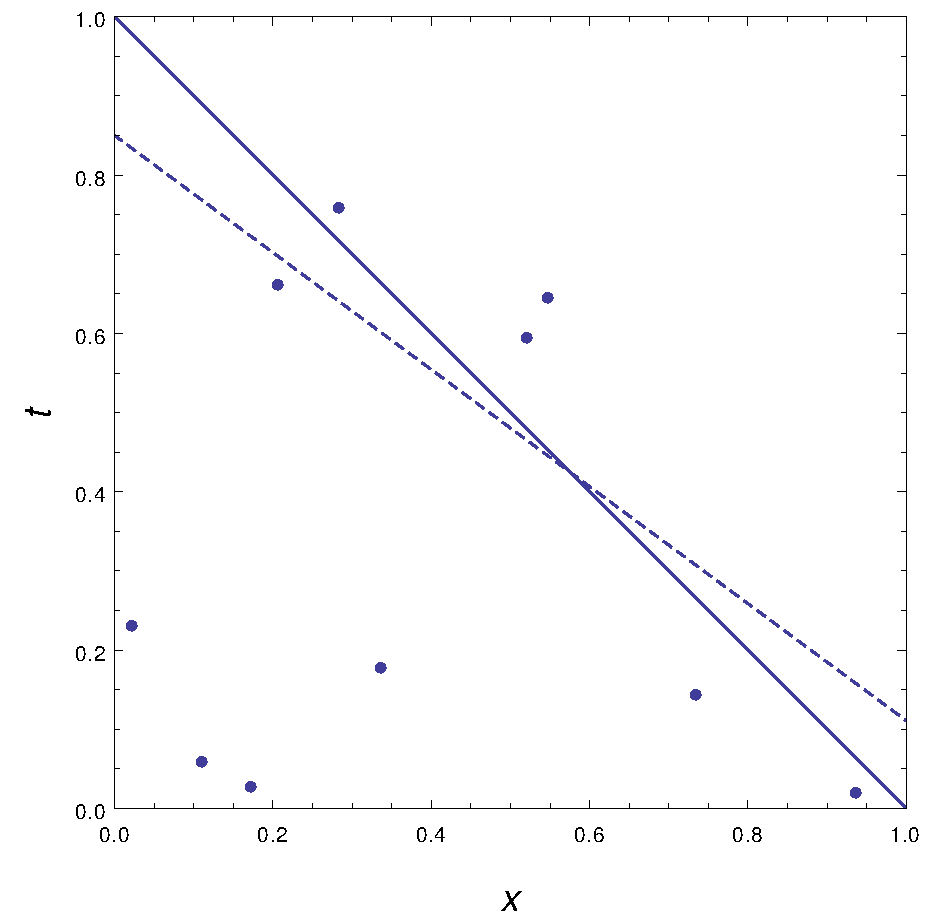
\includegraphics[width=\textwidth]{low_density_sprinkling_with_null_and_spacelike}
                \caption{low density sprinkling}
                \label{fig:low_density_sprinkling_with_null_and_spacelike}
        \end{subfigure}
        \begin{subfigure}[b]{0.49\textwidth}
                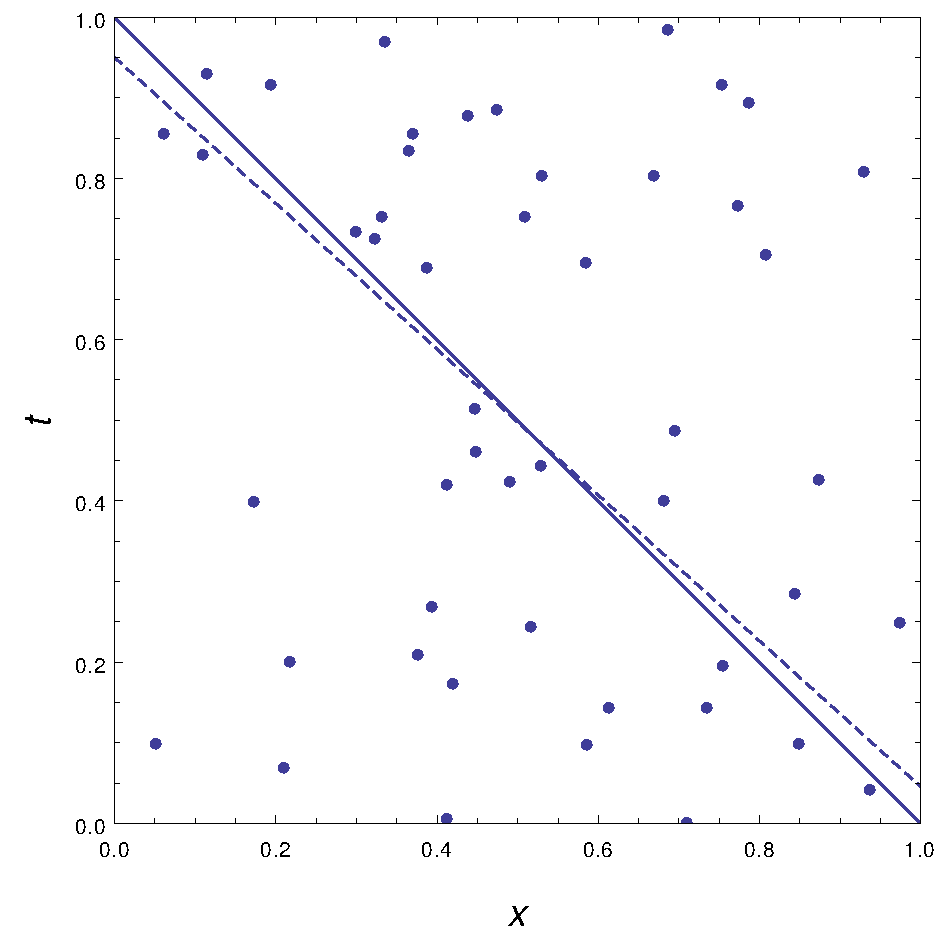
\includegraphics[width=\textwidth]{high_density_sprinkling_with_null_and_spacelike}
                \caption{high density sprinkling}
                \label{fig:high_density_sprinkling_with_null_and_spacelike}
        \end{subfigure}
        \caption{The partition of the causet induced by the surface is unchanged after tilting the surface between null (solid line) and spacelike (dashed line). With an even higher density, as in (b), one can simply tilt the surface by some smaller amount to keep the partition unaltered.}\label{fig:animals}
\end{figure}

Given a causal set with a spacelike partition, there follows a natural definition for the ``immediate neighbours'' in the past and future sets of the partition. The ``immediate neighbours in the past'' of the partition can be defined as those elements of $\mathcal{C}^-$ that have no elements in their causal future in $\mathcal{C}^-$. Such elements will be referred to as \textit{maximal elements} in $\mathcal{C}^-$. We assume an analogous definition for immediate neighbours to the $future$ of the partition, which we shall refer to as \emph{minimal elements} in $\mathcal{C}^+$. Given these definitions, we will see that the intuitive idea for the boundary term as the ``rate of change of spacetime atoms'' across a partition indeed bears out.

In the continuum the GHY term is usually calculated for the future or past bounding surfaces of a manifold, not for a partitioning surface. We wish to calculate the GHY term for future or past boundaries of causets, but there are a couple issues we must deal with. First, if we can faithfully embed a causet $\mathcal{C}$ into $M$ then the boundary surface of $M$ will induce a trivial partition of $\mathcal{C}$ (every element of $\mathcal{C}$ will lie in the bulk of $M$), thus the previous notion of the boundary term as a rate of change of spacetime atoms across a partition does not work. Second, what does it mean to say a bounding surface of a causet if it is not faithfully embeddable in some manifold? Previously if the causet was not faithfully embeddable we could still define the causal set analogue of the surface as a partition of the causet, but now we have that either $\mathcal{C}^+$ or $\mathcal{C}^-$ will be the empty set. The first issue is not a problem, and we will see that a causal set GHY term can be found for a future (past) boundary of $M$ (the manifold that the causet has been faithfully embedded in) via some other expression in terms of the causet. This expression applies to any causet, and so must apply whether or not the causet is faithfully embeddable, but this runs us into the second issue above. What do we mean by a boundary of a causet? If one is given a causet with maximal and/or minimal elements, certain quantities can be calculated for that causet, like the GHY term we will propose in the next section. We will not provide any physical meaning to a \emph{future} or \emph{past boundary} of a causet, and shall merely state that they are abstract objects for which certain causal set quantities can be calculated. The reason we say that these quantities are being evaluated for the future (past) boundary of the causet is that given a causet that is faithfully embeddable in some manifold with future (past) boundary, the values of the quantities in question will agree with those of certain geometrical quantities for the continuum boundary, in some continuum limit of the causal set. We will henceforth mention future/past boundaries of causets only in the context of some quantity being evaluated for them.

\subsection{The Boundary Action Family}

For a given causet $\mathcal C$, let us define the function $\F{k}\left[\mathcal{C}\,\right]$, which counts the number of elements in $\mathcal C$ that have exactly $k$ elements in their future, and the function $\P{k}\left[\mathcal{C}\,\right]$, which counts the number of elements which have exactly $k$ elements in their past. An ``$F_0$ element'' is then a \emph{maximal} element and a ``$P_0$ element'' is a \emph{minimal} element.

Given a causet, $\mathcal{C}$, with a spacelike partition so that $\mathcal C = \mathcal C^+ \cup\, \mathcal C^-$, we propose the following family of functions as the generalised causal set boundary action:
\be\label{general_boundary_sum}
S^{ (d)}_{GHY}\left[\mathcal{C}^-,\mathcal{C}^+;\vec{p}, \vec{q}\,\right]= \left (l/l_p\right)^{d-2} c_{d}
\left ( \sum_m p_m \F{m}\left[\mathcal{C}^- \right]
+  \sum_n q_n \P{n}\left[\mathcal{C}^+ \right]\right)
\ee
where the constant $c_{d}$ only depends on the spacetime dimension and is given by
\be\label{Cn}
c_{d}=\frac{d (d+1)}{ (d+2)}\left(\frac{V_{d-1}}{d}\right)^{\frac{2}{d}},
\ee
$V_d=\pi^{\frac{d}{2}}/\Gamma\left (\frac{d}{2}+1\right)$ denotes the volume of the unit $d$-ball and $\Gamma (t)$ is the gamma function. We have used $\vec{p}$ and $\vec{q}$ to stand for infinite dimensional vectors $ (p_0,...,p_m,..)$ and $ (q_0,...,q_n,..)$ respectively, where all the $p_m,\: q_n \in \mathbb{R}$. These vectors contain a finite number of non-zero entries, corresponding to the coefficients of the different $\F{m}$ and $\P{n}$ terms. We use the summation $\sum_m$ ($\sum_n$) to denote a sum that runs from $0$ to $m_{max}$ ($n_{max}$), where $m_{max}$ ($n_{max}$) is some integer, the value of which depends on the causet $\mathcal{C}^-$ ($\mathcal{C}^+$), for which all $\F{m}\left[\mathcal{C}^- \right]=0$ ($\P{n}\left[\mathcal{C}^+ \right]=0$) for any $m>m_{max}$ ($n>n_{max}$). Finite values for $m_{max}$ and $n_{max}$ will always exist for any finite causet. The vectors must be chosen such that they satisfy the following conditions.
\begin{align}\label{coefficient_relation1}
& \sum_m p_m \frac{\Gamma\left (\frac{1}{d}+m \right)}{m!}  + \sum_n q_n\frac{\Gamma\left (\frac{1}{d}+n \right)}{n!}=0
\\
& \label{coefficient_relation2}\sum_m p_m \frac{\Gamma\left (\frac{2}{d}+m \right)}{m!}  - \sum_n q_n\frac{\Gamma\left (\frac{2}{d}+n \right)}{n!}=1
\end{align}
Any member of the aforementioned family simply corresponds to a choice of the vectors $\vec{p}$ and $\vec{q}$ satisfying the above criteria.

Given a $d$ dimensional, spatially compact Lorentzian manifold, $M$, the family of functions $S^{ (d)}_{GHY}$ (for different $\vec{p}$ and $\vec{q}$) defines a family of random variables in the following way. The process of sprinkling points into $M$ with density $\rho=l^{-d}$ generates a random causet $\mathcal{C}$, and so the functions $\F{k}$ and $\P{k}$ acting on this random causet are now the random variables $\BF{k}$ and $\BP{k}$. These random variables can be substituted into~\eqref{general_boundary_sum} for $\F{k}$ and $\P{k}$ to give the family of random variables, $\textbf{S}^{ (d)}_{GHY}$. These random variables will be functions of $\rho$ and the two parts of the partitioned manifold, $M^{\pm}$, where the dependence of $\BF{k}$ ($\BP{k}$) on the manifold is restricted to $M^-$ ($M^+$). We claim that in the limit of infinite density the expectation value, in the sprinkling process, of $\textbf{S}^{ (d)}_{GHY}$ (for any vectors $\vec{p}$ and $\vec{q}$ satisfying~\eqref{coefficient_relation1} and ~\eqref{coefficient_relation1}) tends to the continuum GHY boundary term for a surface $\Sigma$ that partitions the manifold into $M^+$ and $M^-$:
\be
\lim_{l\rightarrow0}\left\langle\textbf{S}^{ (d)}_{GHY}[M^-,M^+,\rho;\vec{p} , \vec{q}]\right\rangle= \frac{1}{l_p^{d-2}}\int_{\Sigma} d^{d-1}x\: \sqrt{h}\: K\label{eq:mainconjecture}
\ee
where $\langle\cdot\rangle$ denotes the mean over sprinklings and we have explicitly stated the arguments of $\textbf{S}^{ (d)}_{GHY}$. Technically the right hand side of~\eqref{eq:mainconjecture} is equal to ${S}^{(d)}_{GHY}$ ($-{S}^{(d)}_{GHY}$) evaluated for the manifold $M^-$ ($M^+$) with future (past) bounding surface $\Sigma$.

There is a huge amount of freedom that remains in the choice of $\vec{p}$ and $\vec{q}$. One can see that at least two non-zero entries in $\vec{p}$ or $\vec{q}$ are necessary in order to satisfy~\eqref{coefficient_relation1} and~\eqref{coefficient_relation2}. The values of these non-zero entries will unique, but if more than two entries are non-zero this uniqueness is lost. In a finite difference method one can form a discrete derivative in one direction by taking a difference of two values at different points along that direction, and dividing by the distance between them. We are doing something very similar here. The boundary action (in the continuum) is a derivative in one direction, the normal direction (as in~\eqref{eq:normal_deriv_boundary}), and so a finite difference method should be able to approximate this with just two terms. This agrees with the fact that we are able write the discrete boundary action with only two non-zero entries.

We will now mention a few of the simplest looking members of the family that arise from having only two non-zero entries in the vectors $\vec{p}$ and $\vec{q}$. Given a causet, $\mathcal{C}$, with a spacelike partition into $\mathcal C^+$ and $\mathcal C^-$ we define the function $S^{ (d)}_0$ as a particular member of the family in~\eqref{general_boundary_sum}:
\be\label{eq:min_max_simple_formula}
S^{ (d)}_{0}\left[\mathcal{C}^-,\mathcal{C}^+\right]:=S^{ (d)}_{GHY}\left[\mathcal{C}^-,\mathcal{C}^+;\vec{p}_0, -\vec{p}_0\,\right]=\left (l/l_p\right)^{d-2}\frac{c_{d}}{2\Gamma\left (\frac{2}{d} \right)}\left ( \F{0}\left[\mathcal{C}^- \right] - \P{0}\left[\mathcal{C}^+ \right] \right)
\ee
where $\vec{p}_0=\left (\left (2\Gamma\left (\frac{2}{d} \right)\right)^{-1},0,0,...\right)$. This is precisely the rate of change of spacetime atoms previously mentioned, as it is just the difference in minimal elements of $\mathcal{C}^+$ and maximal elements of $\mathcal{C}^-$. This expression is the easiest to employ computationally, and we shall use its random variable counterpart, $\textbf{S}^{ (d)}_{0}\left[M^-,M^+,\rho\right]:=\textbf{S}^{ (d)}_{GHY}\left[M^-,M^+,\rho;\vec{p}_0, -\vec{p}_0\right]$, later when we study the fluctuations of the discrete boundary actions numerically.

If one wants to calculate the GHY boundary term for the future (past) boundary of a single causet, $\mathcal{C}$, then one simply inserts $\mathcal{C}$ into the $\mathcal{C}^-$ ($\mathcal{C}^+$) argument of $S^{ (d)}_{GHY}$ and sets $\vec{q}$ ($\vec{p}$) to the zero vector, $\vec{0}= (0,0,...)$. This renders the $\mathcal{C}^+$ ($\mathcal{C}^-$) argument unnecessary and so one can insert the empty set, $\emptyset$, for convenience. We define the functions for the future and past boundaries respectively as:
\begin{align}\label{eq:future_past_boundary_terms1}
S^{ (d)}_{+}[\mathcal{C}]:= & S^{ (d)}_{GHY}\left[\mathcal{C},\emptyset;\vec{p}_1,\vec{0}\,\right] =\left (l/l_p\right)^{d-2}\frac{c_{d}}{\Gamma\left (\frac{2}{d} \right)}\left ( d\:\F{1}\left[\mathcal{C}\,\right] - \F{0}\left[\mathcal{C}\,\right] \right)
\\
\label{eq:future_past_boundary_terms2}
S^{ (d)}_{-}[\mathcal{C}]:= & S^{ (d)}_{GHY}\left[\emptyset,\mathcal{C};\vec{0},-\vec{p}_1\right] =\left (l/l_p\right)^{d-2}\frac{c_{d}}{\Gamma\left (\frac{2}{d} \right)}\left ( \P{0}\left[\mathcal{C}\,\right] - d\: \P{1}\left[\mathcal{C}\,\right] \right)
\end{align}
where $\vec{p}_1=\left (-\Gamma\left (\frac{2}{d} \right)^{-1},d\:\Gamma\left (\frac{2}{d} \right)^{-1},0,0,...\right)$. In writing down an action for a particular causal set, $\mathcal{C}$, one would write down the Benincasa-Dowker action, $S^{ (d)}_{BD}[\mathcal{C}]$. In addition to this we propose that one could include the boundary terms $S^{ (d)}_{+}[\mathcal{C}]$ and $S^{ (d)}_{-}[\mathcal{C}]$. Explicitly, the total action for a causal set is then given by:
\be\label{eq:total_causet_action}
S^{ (d)}=S^{ (d)}_{BD}+S^{ (d)}_{+}-S^{ (d)}_{-}
\ee
where we have omitted the causet argument, $\mathcal{C}$. There may be contributions from the causal set analogue of timelike boundaries but some results suggest that these are included in $S^{ (d)}_{BD}$.

\subsection{The Surface Volume Family}

We also propose a family of functions for the causal set analogue of spatial volume of the spacelike partition:
\be\label{general_area_sum}
A^{ (d)}[\mathcal{C}^-,\mathcal{C}^+;\vec{p},\vec{q}]=\left (l/l_p\right)^{d-1}b_{d}\left (\sum_m p_m \F{m}\left[\mathcal{C}^- \right] + \sum_n q_n \P{n}\left[\mathcal{C}^+ \right]\right)
\ee
where the constant $b_d$ is given by
\be\label{constant_b_d}
b_d=d\left(\frac{V_{d-1}}{d}\right)^{\frac{1}{d}}
\ee
and we have used similar definitions for the arguments $\vec{p}$ and $\vec{q}$. This time however, the coefficients must satisfy 
\be\label{area_coefficient_relation}
\sum_m p_m \frac{\Gamma\left (\frac{1}{d}+m \right)}{m!}  + \sum_n q_n\frac{\Gamma\left (\frac{1}{d}+n \right)}{n!}=1
\ee
From this relation we can see that only one term is necessary to determine an expression for the discrete surface volume, and that when more than one term is added the coefficients will cease to be unique. Once again we can define a family of random variables, $\textbf{A}^{ (d)}$, which will depend upon the parts of the partitioned manifold, $M^{\pm}$, and the sprinkling density, $\rho$. We make another claim that, in the limit of infinite density, the expectation value of $\textbf{A}^{ (d)}$ in the sprinkling process tends to the spatial volume of the surface $\Sigma$.
\be\label{eq:conjecture_for_area}
\lim_{l\rightarrow0}\left\langle\textbf{A}^{ (d)}[M^-,M^+,\rho;\vec{p} , \vec{q}]\right\rangle= \frac{1}{l_p^{d-1}}\int_{\Sigma} d^{d-1}x\: \sqrt{h}
\ee
where the right hand side is the spatial volume of the surface $\Sigma$. In proving~\eqref{eq:mainconjecture} we will establish the results necessary to prove this claim as well.

By making the same restrictions on the arguments as we did for $S^{ (d)}_{GHY}$, we can find expressions for the causal set analogue of the spatial volume of the future or past boundaries. We define functions for the future and past boundaries respectively as two of the simplest members of the family:
\begin{align}\label{eq:future_past_spatial_volume}
A^{ (d)}_{+}[\mathcal{C}]:=A^{ (d)}[\mathcal{C},\emptyset;\vec{p}_2,\vec{0}]= & \left (l/l_p\right)^{d-1}\frac{b_{d}}{\Gamma\left (\frac{1}{d}\right)}\: \F{0}[\mathcal{C}]
\\
A^{ (d)}_{-}[\mathcal{C}]:=A^{ (d)}[\emptyset,\mathcal{C};\vec{0},\vec{p}_2]= & \left (l/l_p\right)^{d-1}\frac{b_{d}}{\Gamma\left (\frac{1}{d}\right)}\: \P{0}[\mathcal{C}]
\end{align}
where $\vec{p}_2= (\Gamma\left (\frac{1}{d}\right)^{-1},0,0,...)$.

%\begin{figure}
%  \centering
%    {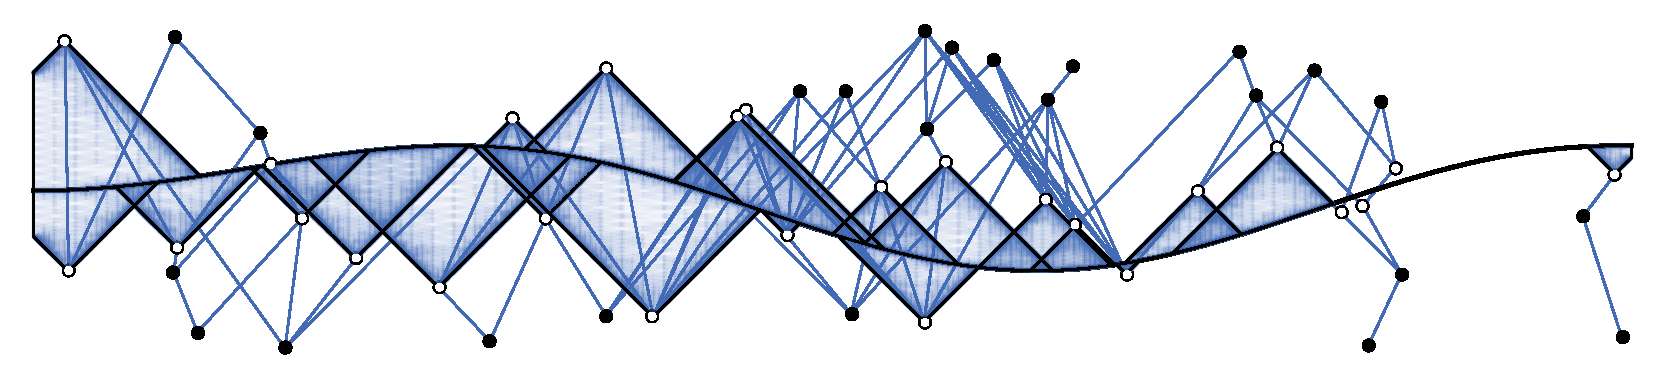
\includegraphics[width=\textwidth]{minmaxplot}}
%     \caption{An illustration of the idea. Pictured %here is a causal set obtained by a sprinkling into a %spacetime partitioned by a spacelike hypersurface. %The minimal and maximal points about the surface are %highlighted and the shaded regions illustrate the %regions whose volumes $V_\blacktriangle$ and %$V_\blacktriangledown$ are needed in the proof.}
%     \label{fig:Nmin_Nmax}
%*\end{figure}

\section{The Proof}

\subsection{$\left\langle \BF{m}\right\rangle$ and $\left\langle \BP{m}\right\rangle$ for Poisson Sprinklings}

In order to prove~\eqref{eq:mainconjecture} and~\eqref{eq:conjecture_for_area} let us first derive expressions for the mean values of $\BF{m}$ and $\BP{m}$. The proof will follow almost automatically, as~\eqref{general_boundary_sum} and~\eqref{general_area_sum} are just linear combinations of $\F{m}$ and $\P{m}$ terms, and thus the mean values of the random variable counterparts for~\eqref{general_boundary_sum} and~\eqref{general_area_sum} will just be linear combinations of $\left\langle \BF{m}\right\rangle$ and $\left\langle \BP{m}\right\rangle$ terms.

For any instance of the sprinkling, the probability that a sprinkled point $p\in M$ below the surface $\Sigma$ is an $F_k$ element is given by the probability that $k$ points of the sprinkling lie in the region $J^{+} (p)\cap J^{-} (\Sigma)$, the intersection of the causal future of $p$ with the causal past of the surface $\Sigma$.\footnote{For notational convenience we use the symbol $x$ to refer to the causal element $x\in\mathcal C$, to its embedding in the manifold $M$, and to its coordinates in some chart on $M$.} This region, for some general spacetime, will be the interior of some curvy $d$-dimensional lightcone truncated by the surface $\Sigma$. We will refer to these regions as \emph{truncated cones}. The Poisson process assigns a probability
\be\label{Poisson}
\mathbb P\left (\text{k points in }J^{+} (p)\cap J^{-} (\Sigma)\right)=\frac{\left (\rho\: V_\blacktriangledown (p)\right)^k}{k!}e^{-\rho V_\blacktriangledown (p)}
\ee
to this event, where $V_\blacktriangledown (p):= V (J^{+} (p)\cap J^{-} (\Sigma))$ is the spacetime volume of the region $J^{+} (p)\cap J^{-} (\Sigma)$. The probability of sprinkling an element into an infinitesimal four-volume $dV_p$ at $p$ is $\rho dV_p$ where $\rho=l^{-d}$ is the sprinkling density, and so the total expected number of $\F{k}$ elements below $\Sigma$ is
\be\label{eq:nmax}
\left\langle \BF{k}\right\rangle =\rho\int_{J^{-} (\Sigma)}dV_p\; \frac{\left (\rho\: V_\blacktriangledown (p)\right)^k}{k!}e^{-\rho V_\blacktriangledown (p)}
\ee
Similarly the expected number of $\P{k}$ elements above $\Sigma$ is
\be\label{eq:nmin}
\left\langle \BP{k}\right\rangle =\rho\int_{J^{+} (\Sigma)}dV_p\; \frac{\left (\rho\: V_\blacktriangle (p)\right)^k}{k!}e^{-\rho V_\blacktriangle (p)}
\ee
where $V_\blacktriangle (p):= V (J^{+} (\Sigma)\cap J^{-} (p))$.

In the limit $\rho\rightarrow\infty$, both quantities will diverge, but if some combination of $\P{k}$ and $\F{k}$ grows slower than or at order $\rho^{1-\frac2d}$, the random variable counterpart of the proposed action~\eqref{general_boundary_sum} will tend to a finite value in the continuum limit.

Consider a set of synchronous or Gaussian Normal Coordinates (GNC), $x^\mu= (t,\mathbf x)$, adapted to $\Sigma$ such that in a neighbourhood $U_\Sigma$ of $\Sigma$ the line element is
\be
ds^2 = -dt^2 + h_{ij} (t,\mathbf x) dx^i dx^j.
\ee
In these coordinates, the surface $\Sigma$ corresponds to $t=0$, and the coordinate $t$ measures the proper time elapsed along geodesics whose tangent vector is proportional to the surface normal on $\Sigma$.
%\be\label{GNC_metric}
%g_{\mu\nu} (x)=
%\begin{pmatrix}
 %-1&0 \\
% 0&h_{ij} (x)
%\end{pmatrix}.
%\ee
%In order to find $N_{max}$, the number of maximal points below the surface, one has to use the fact that the points have been sprinkled with a Poisson distribution. 
%If we pick a point $x_0= (0,\mathbf{x})\in \Sigma$ on the surface that has the same spatial coordinates as $x= (t,\mathbf{x})$ then the coordinate time, $t$, is the proper time elapsed along the unique geodesic between $x_0$ and $x$. The volume $V (\Sigma,x)$ then only depends on $t$.~\mb{error?}  
The integrals~\eqref{eq:nmax} and~\eqref{eq:nmin} seem intractable as they stand, since the integration is over the entire causal past/future of the surface and the volume expressions will be complicated in the presence of curvature. However, for large $\rho$ (small $l$), the integrands $\exp (-\rho V)$ will be exponentially suppressed unless the volumes are small. Consider the spacetime region $U_\varepsilon=\left\{|t|<\varepsilon\right\}$ around the surface $\Sigma$ for some $\varepsilon>0$ (with $\varepsilon$ small enough such that the GNC system is valid throughout $U_\varepsilon$). We will assume that for any such $\varepsilon$, the contribution from points with $|t|>\varepsilon$ to the integrals~\eqref{eq:nmax} and \eqref{eq:nmin} can be made arbitrarily small by setting $\rho$ large enough, since the volumes of the truncated past/future lightcones for such points will be too large. Hence, as $\rho\rightarrow\infty$, the integration ranges in \eqref{eq:nmax} and \eqref{eq:nmin} can be cut off at finite time $t=\pm\varepsilon$ with $\varepsilon$ arbitrarily small, which allows us to expand the time integration-variable about zero. These assumptions of course impose certain regularity conditions on the surface $\Sigma$, but so long as $\Sigma$ is a closed compact manifold and is everywhere spacelike then all we require is that the radius of extrinsic curvature, $R$, satisfies $R\gg l$. The integrals then simplify to
\begin{gather}\label{eq:nmax_and_eq:nmin}
\begin{aligned}
\left\langle \BF{k}\right\rangle & =\rho \int_{\Sigma}d^{d-1}x\int_{-\varepsilon}^{0}dt\:
h^{\frac{1}{2}}\left (1+
\frac{1}{2}\frac{\dot{h}}{h}t+O (t^2)\right)
 \frac{\left (\rho\: V_\blacktriangledown (p)\right)^k}{k!} e^{-\rho V_\blacktriangledown (t,\mathbf x)}
\\
\left\langle \BP{k}\right\rangle & =\rho \int_{\Sigma}d^{d-1}x\int_{0}^{\varepsilon}dt\:
h^{\frac{1}{2}}\left (1+
\frac{1}{2}\frac{\dot{h}}{h}t+O (t^2)\right) \frac{\left (\rho\: V_\blacktriangle (p)\right)^k}{k!} e^{-\rho V_\blacktriangle (t,\mathbf x)}
\end{aligned}
\end{gather}
where $h:= det\left (h_{ij} (0,\mathbf{x})\right)$ and $\dot{}\: := \frac{\partial}{\partial t}$ and the metric determinant has been in expanded in small $t$.

\subsection{Lightcone Volumes}

In order to evaluate the volume $V_\blacktriangledown (p)$ or $V_\blacktriangle (p)$ of a truncated cone we will perform a coordinate transformation to Riemann Normal Coordinates (RNCs) in a neighbourhood containing the cone. The volumes can be expressed by series expansions in $t$. We will only need to retain up to order $O(t^{d+1})$ as higher order terms will be shown to vanish when we take the limit of $\rho\rightarrow\infty$ on the mean values of~\eqref{general_boundary_sum} and~\eqref{general_area_sum}. Henceforth, whenever we state that a term of some order vanishes in the limit we mean that it vanishes in the way just stated. The discussion for the two volume integrals is identical so we will only outline it for $V_\blacktriangle (p)$ (i.e. for points to the future of $\Sigma$).

Fix $p\in M$ and denote its coordinate values in GNCs by $x^\mu_p= (t_p,\mathbf x_p)$. It will be convenient to use RNCs centered not at the tip, $p$, of the cone but instead at the point $p_0$ where the unique geodesic through $p$ whose tangent is normal to $\Sigma$ intersects $\Sigma$. In GNCs this simply corresponds to the point $p_0$ with coordinates $x_0^\mu=x^\mu (p_0)= (0,\mathbf x_p)$. RNCs centered at $p_0$ will be given the symbol $y^{\overline{\mu}}$, or in terms of coordinates as $(y^{\overline{0}},\mathbf{y})=(\overline{t},\mathbf{y})$.
%\mb{let's put all facts about $x^\mu$ and $y^{\overline\mu}$ for $p$ and $p_0$ here and expansion of det in RNC.} 
We need to assume that for any $p$ in $U_\varepsilon$, the Riemann normal neighbourhood $U_p\subset M$ (throughout which the RNC system centered at $p_0$ is well-defined) contains the truncated cone $J^- (p)\cap J^+ (\Sigma)$. This assumption seems reasonable given the that $U_\varepsilon$ can be made arbitrarily ``thin'' as $\rho\rightarrow\infty$. In RNCs the metric and the Christoffel symbols at $p_0$ are those of flat space:
\be\label{eq:RNCMetricTransAtPAndChris}
g_{\overline{\mu} \overline{\nu}} (p_0)=\eta_{\overline{\mu} \overline{\nu}}=A^{\mu}_{\;\overline{\mu}}A^{\nu}_{\;\overline{\nu}}g_{\mu\nu} (p_0)\;,\;\;\;\;\Gamma^{\overline{\mu}}_{\;\overline{\nu}\overline{\rho}} (p_0)=0
\ee
The $A^{\mu}_{\;\overline{\mu}}$ govern the coordinate transformation from GNCs to RNCs to linear order. %but $O (x^2)$ corrections may be required. 
To second order the coordinate transformation is given by
\be\label{eq:RNCtotaltrans}
y^{\overline{\mu}}=A^{\overline{\mu}}_{\;\nu}x^\nu+\frac{1}{2}A^{\overline{\mu}}_{\;\mu}\Gamma^{\mu}_{\;\nu\rho} (p_0)x^\nu x^\rho+O ( (x-x_0)^3).
\ee
The inverse relation to first order is 
\be\label{eq:RNCinversetrans}
x^{\mu}=A^{\mu}_{\;\overline{\nu}}y^{\overline{\nu}}+O (y^2)
\ee
and one finds that the $A^{\mu}_{\;\overline{\mu}}$ must satisfy
\be\label{eq:RNCeqnforA}
A^{\overline{\mu}}_{\;\mu}A^{\mu}_{\;\overline{\nu}}=\delta^{\overline{\mu}}_{\;\overline{\nu}}\;,\;\;\;\;A^{\mu}_{\;\overline{\mu}}A^{\overline{\mu}}_{\;\nu}=\delta^{\mu}_{\;\nu}
\ee
Let us denote the time-coordinate of $p$ in GNCs by $T=x^0_p=t_p$. For the transformation from GNCs to RNCs at $p_0$ one finds that $A^{\overline 0}_{\;0}=1$, $A^{\overline 0}_{\;i}=0$ and $\delta_{\ibar\jbar}=A^i_{\;\ibar}A^j_{\;\jbar}h_{ij} (p_0)$, which in particular implies $y^{\overline{0}}_p=\overline{t}_p=t_p=T$.

Now the volume of the truncated cone can be found as follows. 
%Consider the past lightcone emanating at the point $p_0= (T,\mathbf x_0)$ truncated by $\Sigma$. There is a unique point $q_0= (0,\mathbf x_0)$ on $\Sigma$ associated with $p_0$, separated from $p_0$ by proper time $T$. 
The volume of the cone is given by
\be\label{eq:VolumeWithNoSimplifications}
V_\blacktriangle (p)=\int_{\mathcal{X}_p} d^d x\;\sqrt{-g}
\ee
where the integration region, $\mathcal{X}_p:= J^- (p)\cap J^+ (\Sigma)$ will be a complicated expression. In RNC one can expand the metric determinant in~\eqref{eq:VolumeWithNoSimplifications} to find
\be\label{eq:VolumeWithRNC}
V_\blacktriangle (p) =\int_{\mathcal{X}_p}d^dy+\int_{\mathcal{X}_p}d^dy\left (-\frac{1}{6}R_{\overline{\mu}\overline{\nu}} (p_0)y^{\overline{\mu}}y^{\overline{\nu}} \right)+O (T^{d+3})
\ee
where $R_{\overline{\mu}\overline{\nu}} (p_0)$ is the Ricci tensor in RNC evaluated at $p_0$. The second integral comes in at $O (T^{d+2})$ so the volume may be written as
\be\label{eq:VolumeToLowestOrder}
V_\blacktriangle (p) =\int_{\mathcal{X}_p}d^dy+O (T^{d+2})
\ee
Terms of $O (T^{d+2})$ can be retained till the end, but we will prove that they vanish in the limit.

This is now a simple volume integral but we need to find the boundaries of $\mathcal{X}_p$ to write down the integration limits. There are two parts to the boundary of the (solid) truncated cone: the \emph{base}, defined as $B(p):=\Sigma\cap J^-(p)$, and the \emph{top} defined as the set corresponding to the lightcone emanating at $p$ with all points below $\Sigma$ removed, written as $T(p):=\partial J^-(p)\setminus\partial(J^-(p)\cap (J^-(\Sigma)\setminus\Sigma))$. Now the boundary of $\mathcal{X}_p$ is simply $\partial\mathcal{X}_p=B(p)\cup T(p)$. First we look at the top. Following \cite{Khetrapal_Sumati:Causal_Diamond_Volume} it can be shown that the first curvature correction to the lightcone volume comes in at $O (T^{d+2})$ and so can be ignored for our purposes. This means that the top can be treated as an effectively flat lightcone in RNCs and thus it corresponds to the set of points satisfying $ (y^{\overline{1}})^2+ (y^{\overline{2}})^2+...+ (y^{\overline{d-1}})^2= T-\overline{t}$ where the coordinates  $y^{\overline{i}}$ run from $0$ up to some maximum at the points where the flat cone meets the surface $\Sigma$.

The base of the cone in GNCs is simply a part of the surface $t=0$, so we can use (\ref{eq:RNCtotaltrans}) to find the equation for the surface in RNCs. Equation (\ref{eq:RNCtotaltrans}) gives
\be\label{eq:BottomSurfaceWithGNC}
\overline{t}=\frac{1}{2}\Gamma^{0}_{\;ij} (p_0)x^i x^j+O ( x^3)
\ee
The linear part on the right of (\ref{eq:RNCtotaltrans}) vanishes as $A^{\overline{0}}_{\;\mu}x^{\mu}=x^0$ (as $A^{\overline{0}}_{\;i}=0$ and $A^{\overline{0}}_{\;0}=1$) and $x^0=t=0$ for the bottom surface. Using the inverse RNC relation (\ref{eq:RNCinversetrans}) one can find the equation for the bottom surface in RNCs:
\be\label{eq:BottomSurface}
\overline{t}=\frac{1}{2}\Gamma^{0}_{\;ij} (p_0)A^{i}_{\;\ibar}A^{j}_{\;\jbar}y^{\ibar} y^{\jbar}+O (y^3)
\ee
Let us rewrite this equation in spherically symmetric coordinates, i.e. define $r:=\sqrt{\delta_{\ibar\jbar}y^\ibar y^\jbar}$ and the usual angular coordinates $\phi_1,..,\phi_{d-2}$ in terms of the spatial coordinates $y^{\overline{1}} = r \cos (\phi_1),\ldots, y^{\overline{d-1}} = r \sin (\phi_1) \cdots \sin (\phi_{d-3}) \sin (\phi_{d-2})$. Then
\be\label{eq:RadialBottomSurface}
\overline{t}=\frac{1}{2}\left (\Gamma^{0}_{\;ij} (p_0)A^{i}_{\;\ibar}A^{j}_{\;\jbar}\frac{y^{\ibar} y^{\jbar}}{r^2}\right)r^2+O (y^3)=\frac{1}{2}f (\mathbf{x}_p,{\boldsymbol\phi})r^2+O (y^3)
\ee
where $\boldsymbol\phi$ stands collectively for all the angular coordinates $\phi_1,..,\phi_{d-2}$. The function $f (\mathbf{x}_p,\boldsymbol\phi)$ depends on $\mathbf{x}_p$ since $\Gamma^{0}_{\;ij}$ and $A^{i}_{\;\ibar}$ depend on $p_0$.
%One can see that $f (\mathbf{x}_0,\boldsymbol\phi)$ depends on the angles, $\phi$, by substituting the relations below into (\ref{eq:RadialBottomSurface})
%\begin{equation}
%\begin{aligned}\label{eq:SphericalCoords}
%y^{\overline{1}} &= r \cos (\phi_1)  \\
%y^{\overline{2}} &= r \sin (\phi_1) \cos (\phi_2)  \\
%y^{\overline{2}} &= r \sin (\phi_1) \sin (\phi_2) \cos (\phi_3)  \\
%    &\vdots  \\
%y^{\overline{d-2}} &= r \sin (\phi_1) \cdots \sin (\phi_{d-3}) \cos (\phi_{d-2})  \\
%y^{\overline{d-1}} &= r \sin (\phi_1) \cdots \sin (\phi_{d-3}) \sin (\phi_{d-2})
%\end{aligned}
%\end{equation}

With the boundaries of the integration region in place, we can now write down the integral explicitly in spherical coordinates:
\be\label{eq:VolumeIntegralSpherical}
V_\blacktriangle (p)=\int_{S^{d-2}}
d\Omega_{d-2}
\int_{0}^{r_{max} (\phi)}r^{d-2}dr
\int_{\frac{1}{2}f (\mathbf{x}_p,\phi)r^2}^{-r+T}
d\overline{t}+O (T^{d+2})
\ee
where $r_{max} (\boldsymbol\phi)$ is the value of the radial coordinate for which the base intersects the top at an angle $\boldsymbol\phi$, as shown in Figure \ref{fig:cone_plot}. To find this value we equate the time coordinates of the top and base surfaces to give 
\be
\frac{1}{2}f (\mathbf{x}_p,\boldsymbol\phi){r_{max}}^2 (\boldsymbol\phi)=-r_{max} (\boldsymbol\phi)+T
\ee 
We then solve this for $r_{max} (\boldsymbol\phi)$ and take the positive solution. The solution can be expanded in $T$ and is simply $r_{max}=T+O (T^2)$, with angular dependent terms contributing at $O (T^2)$. The $O (T^2)$ term will contribute at $O (T^{d+2})$ in the volume integral and so can be ignored. Substituting $r_{max}=T$ into (\ref{eq:VolumeIntegralSpherical}) allows us to evaluate the integral, wherein we find 
\begin{figure}[t]
  \centering
    {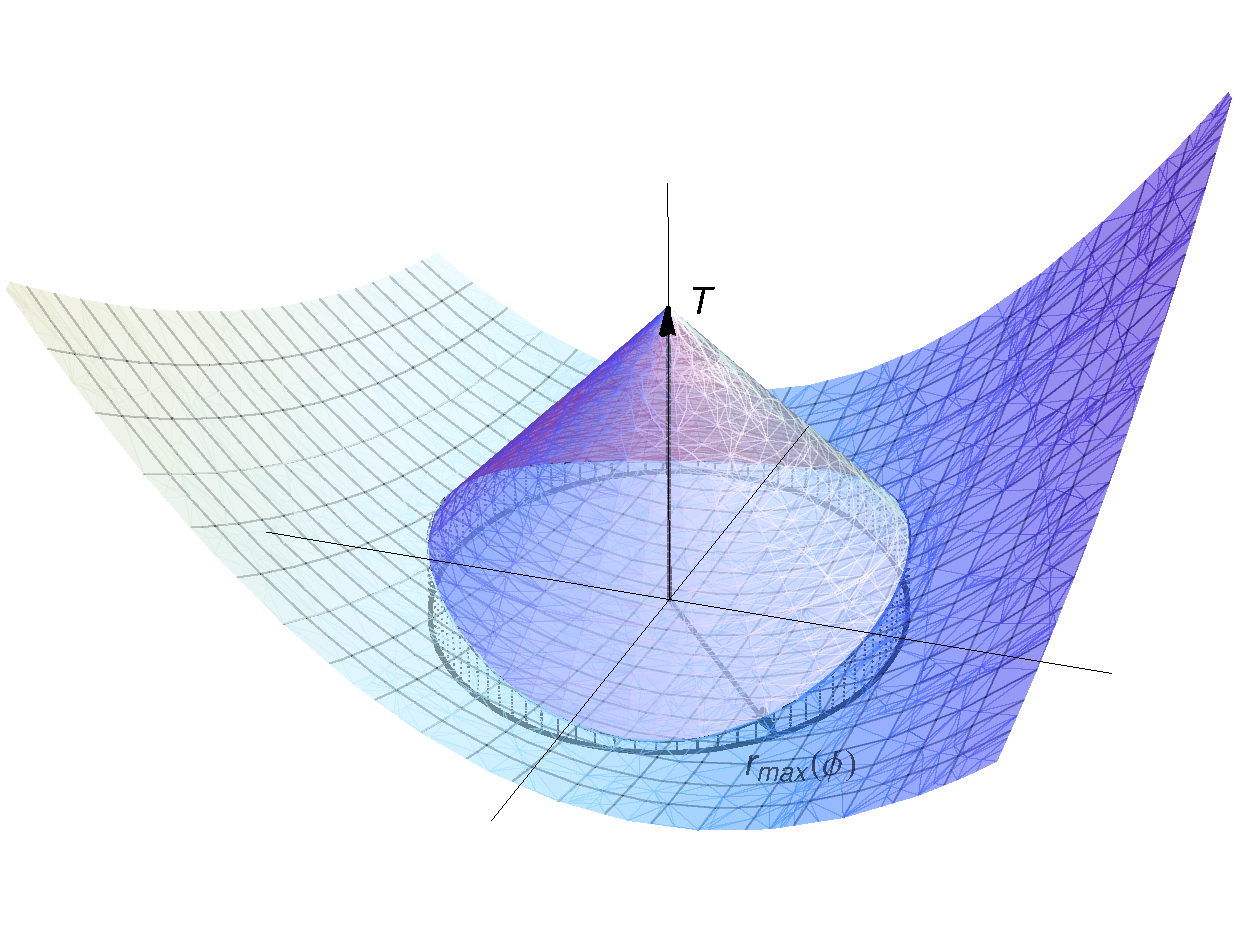
\includegraphics[scale=0.5]{coneplot}}
     \caption{A $3$-dimensional representation of the region $\mathcal{X}_p$ in RNCs. The top part of $\partial\mathcal{X}_p$ can be approximated as a flat cone, and the base surface intersects the top part at a radial coordinate, $r_{max} (\boldsymbol\phi)$, which will in general be a function of the angles $\boldsymbol\phi$ (in $3$-dimensions there is one angle $\phi$). This function is found by projecting down from the intersection to the $\overline{t}$ plane. The size of the region inside the top and bottom bounding surfaces is the volume we want to calculate.}
     \label{fig:cone_plot}
\end{figure}
\be\label{eq:VolumeNoK}
V_\blacktriangle (p)
=\frac{V_{d-1}}{d}T^d\left (1-\frac{d}{2 (d+1)}\Gamma^{0}_{\;ij} (p_0)A^{i}_{\;\ibar}A^{j}_{\;\jbar}\delta^{\ibar\jbar}T\right)
+O (T^{d+2})
\ee
where the $\delta^{\ibar\jbar}$ comes from the fact that cross terms ($\ibar\neq \jbar$) vanish under the angular integration. The defining relations for $A^{i}_{\;\ibar}$ can now be rearranged to give $A^{i}_{\;\ibar}A^{j}_{\;\jbar}\delta^{\ibar\jbar}=h^{ij} (p_0)$. In GNCs the extrinsic curvature on the surface is given by
\be\label{eq:K}
K
=g^{\mu\nu }\nabla_{\mu}n_{\nu}
=-\Gamma^{0}_{\;ij}h^{ij}=-\frac{1}{2}\frac{\dot{h}}{h}.
\ee
Substituting this into~\eqref{eq:VolumeNoK} we obtain 
\begin{align}
V_\blacktriangle (T,\mathbf x)
&=\frac{V_{d-1}}{d}T^d\left (1+\frac{d}{2 (d+1)}K (0,\mathbf{x})T\right)
+O (T^{d+2}) \label{eq:TopVolumeWithK}\\
V_\blacktriangledown (-T,\mathbf x)
&=\frac{V_{d-1}}{d}T^d\left (1-\frac{d}{2 (d+1)}K (0,\mathbf{x})T\right)
+O (T^{d+2}), \label{eq:BottomVolumeWithK}
\end{align}
having dropped the subscript $p$. Given the volume expressions in GNCs we now proceed to evaluate the integrals for $\left\langle \BP{k}\right\rangle$ and $\left\langle \BF{k}\right\rangle$.

\subsection{The mean of $\textbf{S}^{ (d)}_{GHY}\left[\mathcal {C}^-,\mathcal{C}^+;\vec{p},\vec{q}\,\right]$}

Using the previous equations for the volumes of the truncated cones we find that~\eqref{eq:nmax_and_eq:nmin} reduces to
\begin{gather}\label{eq:nmax_and_eq:nmin_volume_expanded}
\begin{aligned}
\left\langle \BF{k}\right\rangle = \frac{\rho^{k+1}}{k!} & \int_{\Sigma}d^{d-1}x\int_{-\varepsilon}^{0}dt\:
h^{\frac{1}{2}}\left (1+
\frac{1}{2}\frac{\dot{h}}{h}t\right)
 \\
 & \times \Big ( A (-t)^d \Big)^k 
 \Big ( 1 - B (-t) \Big)^k
 e^{-\rho A (-t)^d \left[1-B (-t) \right]} + .\,.\,.
\\
\left\langle \BP{k}\right\rangle = \frac{\rho^{k+1}}{k!} & \int_{\Sigma}d^{d-1}x\int_{0}^{\varepsilon}dt\:
h^{\frac{1}{2}}\left (1+
\frac{1}{2}\frac{\dot{h}}{h}t\right)
 \\
 & \times \Big ( A\: t^d \Big)^k 
 \Big ( 1 + B\: t \Big)^k
 e^{-\rho A\: t^d \left[1+B\: t \right]} + .\,.\,.
\end{aligned}
\end{gather}
where we have defined
\begin{gather}\label{A_and_B_defn}
\begin{aligned}
A & := \frac{V_{d-1}}{d} \\
B & := \frac{V_{d-1}}{2 (d+1)}K (0,\mathbf{x})
\end{aligned}
\end{gather}
Once again the higher order terms that have been ignored in both equations will be shown to vanish in the limit. From~\eqref{eq:K} we can substitute $K$ in for $-\frac{1}{2}\frac{\dot{h}}{h}t$. We swap the integration variable from $t\rightarrow -t$ in the first equation and expand the $O (t^{d+1})$ part of the exponentials to give
\begin{gather}\label{eq:nmax_and_eq:nmin_volume_expo_expanded}
\begin{aligned}
\left\langle \BF{k}\right\rangle = \frac{\rho^{k+1}}{k!} & \int_{\Sigma}d^{d-1}x\int_{0}^{\varepsilon}dt\:
h^{\frac{1}{2}}\left (1+
K\: t\right)
 \\
 & \times \Big ( A\: t^d \Big)^k 
 \Big ( 1 - B\: t \Big)^k
 \Big ( 1 + \rho A B\: t^{d+1} \Big)
 e^{-\rho A\: t^d} + .\,.\,.
\\
\left\langle \BP{k}\right\rangle = \frac{\rho^{k+1}}{k!} & \int_{\Sigma}d^{d-1}x\int_{0}^{\varepsilon}dt\:
h^{\frac{1}{2}}\left (1-
Kt\right)
 \\
 & \times \Big ( A\: t^d \Big)^k 
 \Big ( 1 + B\: t \Big)^k
  \Big ( 1 - \rho A B\: t^{d+1} \Big)
 e^{-\rho A\: t^d} + .\,.\,.
\end{aligned}
\end{gather}
The reason for expanding the exponentials is that the integrals will have to be put into the form of Gaussian integrals in order to evaluate them in the limit $\rho\rightarrow\infty$. The above expressions are almost the same apart from a few sign differences, so from now on we will just work with the expression for $\left\langle \BP{k}\right\rangle$. By expanding the brackets, and retaining only necessary orders, the integral can be split into two parts of differing powers of $\rho$.
\begin{gather}\label{eq:n_min_different_rho_terms}
\begin{aligned}
\left\langle \BP{k}\right\rangle & = \frac{\rho^{k+1}A^k}{k!}\int_{\Sigma}d^{d-1}x\: h^{\frac{1}{2}}\int_{0}^{\varepsilon}dt\:
\left[ \left ( t^{dk} + \left (kB-K \right)t^{dk+1}\right) + O\left (t^{dk+2}\right) \right] e^{-\rho A\: t^d}
 \\
 & - \frac{\rho^{k+2}A^{k+1}}{k!}\int_{\Sigma}d^{d-1}x\: h^{\frac{1}{2}}\int_{0}^{\varepsilon}dt\:
\left[ Bt^{dk+d+1} + O\left (t^{dk+d+2}\right) \right] e^{-\rho A\: t^d}
\end{aligned}
\end{gather}
To find out how this diverges in the limit of $\rho \rightarrow\infty$, it suffices to find the divergence of the following general expression
\be\label{eq:general_t_n_integral}
\lim_{\rho\rightarrow\infty}\rho^{p}\int_{0}^{\varepsilon}dt\
t^{q}e^{-\rho At^{d}}
\ee
where $p,q \in \mathbb{R}$. We make the substitution $z=\rho At^{d}$ to put~\eqref{eq:general_t_n_integral} into the form of an incomplete gamma function.
\be\label{eq:incomplete_gamma_function}
\lim_{\rho\rightarrow\infty}\frac{A^{-\left (\frac{q+1}{d} \right)}}{d}\rho^{p-\left (\frac{q+1}{d} \right)}\int_{0}^{\rho A \varepsilon^d}dz\
z^{\left (\frac{q+1}{d} \right)-1}e^{-z}
\ee
The pre-factor has come from the substitution. In the limit we can retain the $\rho$ outside the integral while taking the integration limit to $\infty$. In doing this the integral becomes a gamma function.
\be\label{eq:gamma_function}
\lim_{\rho\rightarrow\infty}\frac{A^{-\left (\frac{q+1}{d} \right)}}{d}\rho^{p-\left (\frac{q+1}{d} \right)}\int_{0}^{\infty}dz\
z^{\left (\frac{q+1}{d} \right)-1}e^{-z}=\lim_{\rho\rightarrow\infty}
\frac{A^{-\left (\frac{q+1}{d} \right)}}{d}\rho^{p-\left (\frac{q+1}{d} \right)}\Gamma\left ( \frac{q+1}{d} \right)
\ee
We can use this procedure to take the limit of~\eqref{eq:n_min_different_rho_terms} and formulate the answer in terms of gamma functions. The limits of both $\left\langle \BF{k}\right\rangle$ and $\left\langle \BP{k}\right\rangle$ are then given by
\begin{gather}\label{eq:nmax_nmin_final}
\begin{aligned}
\lim_{\rho\rightarrow\infty}\left\langle \BF{k}\right\rangle = \lim_{\rho\rightarrow\infty} & \left[ \rho^{1-\frac{1}{d}} \left (b_d\right)^{-1} \frac{\Gamma\left (\frac{1}{d}+k\right)}{k!}
\int_{\Sigma}d^{d-1}x\: \sqrt{h} \right.
 \\
 &  \left. +\rho^{1-\frac{2}{d}} \left (c_d\right)^{-1} \frac{\Gamma\left (\frac{2}{d}+k\right)}{k!}
\int_{\Sigma}d^{d-1}x\: \sqrt{h}K + O\left (\rho^{1-\frac{3}{d}} \right) \right]
\\
\lim_{\rho\rightarrow\infty}\left\langle \BP{k}\right\rangle = \lim_{\rho\rightarrow\infty} & \left[ \rho^{1-\frac{1}{d}} \left (b_d\right)^{-1} \frac{\Gamma\left (\frac{1}{d}+k\right)}{k!}
\int_{\Sigma}d^{d-1}x\: \sqrt{h} \right.
 \\
 &  \left. -\rho^{1-\frac{2}{d}} \left (c_d\right)^{-1} \frac{\Gamma\left (\frac{2}{d}+k\right)}{k!}
\int_{\Sigma}d^{d-1}x\: \sqrt{h}K + O\left (\rho^{1-\frac{3}{d}} \right) \right]
\\
\end{aligned}
\end{gather}

These objects diverge as $\rho^{1-\frac{1}{d}}$ in the limit. The factor of $\rho$ that must be included in the formula for the surface volume is exactly the inverse of this ($\rho^{\frac{1}{d}-1}$), as can be seen from~\eqref{general_area_sum}, if one substitutes in $l=\rho^{-\frac{1}{d}}$. If we include this factor above, and take the limit, we see that the only remaining terms are proportional to the surface volume. The other terms all have negative powers of $\rho$ and therefore vanish as $\rho\rightarrow\infty$. We can take the mean and limit of $\textbf{A}^{ (d)}$ and substitute in the above expressions to find
\begin{gather}\label{eq:area_final_proof}
\begin{aligned}
\lim_{\rho\rightarrow\infty} & \left\langle \textbf{A}^{ (d)}\right\rangle = \lim_{\rho\rightarrow\infty} \frac{\rho^{\frac{1}{d}-1}}{l_p^{d-1}} b_{d}\left (\sum_m p_m \left\langle\textbf{F}_m\right\rangle  + \sum_n q_n \left\langle\textbf{P}_n\right\rangle\right)
\\
= & \lim_{\rho\rightarrow\infty}\Bigg[ \frac{1}{l_p^{d-1}} \left(\sum_m p_m \frac{\Gamma\left (\frac{1}{d}+m \right)}{m!}  + \sum_n q_n\frac{\Gamma\left (\frac{1}{d}+n \right)}{n!} \right) \int_{\Sigma}d^{d-1}x\: \sqrt{h}+O(\rho^{-\frac{1}{d}})\Bigg]
\\
= & \frac{1}{l_p^{d-1}}\int_{\Sigma}d^{d-1}x\: \sqrt{h}
\end{aligned}
\end{gather}
Where the last line is only true if the vectors, $\vec{p}$ and $\vec{q}$ satisfy~\eqref{area_coefficient_relation}. This concludes the proof of the spatial volume claim,~\eqref{eq:conjecture_for_area}. 

We can also take the mean and limit of $\textbf{S}^{ (d)}_{GHY}$ to find
\begin{gather}\label{eq:boundary_final_proof}
\begin{aligned}
\lim_{\rho\rightarrow\infty} & \left\langle \textbf{S}^{ (d)}_{GHY}\right\rangle = \lim_{\rho\rightarrow\infty} \frac{\rho^{\frac{2}{d}-1}}{l_p^{d-2}} c_{d}\left (\sum_m p_m \left\langle\textbf{F}_m\right\rangle  + \sum_n q_n \left\langle\textbf{P}_n\right\rangle\right)
\\
= & \lim_{\rho\rightarrow\infty}\Bigg[\frac{\rho^{\frac{1}{d}}}{l_p^{d-1}}\frac{c_d}{b_d}\left(\sum_m p_m \frac{\Gamma\left (\frac{1}{d}+m \right)}{m!}  + \sum_n q_n\frac{\Gamma\left (\frac{1}{d}+n \right)}{n!} \right) \int_{\Sigma}d^{d-1}x\: \sqrt{h}
\\
& +\frac{1}{l_p^{d-2}}\left(\sum_m\frac{\Gamma\left (\frac{2}{d}+m \right)}{m!}  - \sum_n q_n\frac{\Gamma\left (\frac{2}{d}+n \right)}{n!} \right) \int_{\Sigma}d^{d-1}x\: \sqrt{h}K + O(\rho^{-\frac{1}{d}})\Bigg]
\\
& = \frac{1}{l_p^{d-2}}\int_{\Sigma}d^{d-1}x\: \sqrt{h}K
\end{aligned}
\end{gather}
Where the last line is true only if the vectors $\vec{p}$ and $\vec{q}$ satisfy~\eqref{coefficient_relation1} and~\eqref{coefficient_relation2}. The proof of~\eqref{eq:mainconjecture} is now complete.

The form of~\eqref{eq:nmax_nmin_final} seems to suggest that $\left\langle \BF{k}\right\rangle$ and $\left\langle \BP{k}\right\rangle$ can be written in terms of a series expansion in reducing powers of $\rho$. Written in terms of the discreteness scale, $l$, it is a Laurent series starting at $l^{1-d}$. The higher order terms, in $l$, will possibly be proportional to higher order normal derivatives of the surface volume. If this were true then one could find causal set versions for the normal derivatives of the surface volume to any order. The exact form of the constant in the next term of the series is unknown and more work must be done to determine a general trend for the constants, and hence find the general series.

\section{Fluctuations}
So far we have only talked about the mean of the causal set boundary action. Let us now turn to its fluctuations (the standard deviation) $\sigma[\textbf{S}^{ (d)}_{GHY}]=\text{Var}[\textbf{S}^{ (d)}_{GHY}]^\frac12$.\footnote{Whenever we say fluctuations we refer to the standard deviation of the random variable, not to its variance.} We can make a heuristic argument to estimate the dependence of fluctuations on $\rho=l^{-d}$. In any spacetime region of fixed volume $V$ the number of causal set elements in a sprinkling is a random variable, $\textbf{N}$, with mean $\left\langle\textbf{N}\right\rangle=\rho V$, and Poisson fluctuations of order $\sqrt{\left\langle\textbf{N}\right\rangle}$. We will use $\textbf{S}^{ (d)}_{0}$ for the boundary action, as it is the simplest case in which to make this argument for the fluctuations. We believe this choice is valid as the simulations have suggested that all members of the $\textbf{S}^{ (d)}_{GHY}$ family have similar fluctions. Since $\BF{0}$ and $\BP{0}$ are random variables associated with a codimension-1 surface (they count elements ``near" $\Sigma$), we may expect their mean values to scale like $\left\langle\textbf{N}\right\rangle^\frac{d-1}{d}$ --- which agrees with the leading order behaviour of~\eqref{eq:nmax_nmin_final} --- and hence that they inherit fluctuations of order $\left\langle\textbf{N}\right\rangle^\frac{d-1}{2d} = (\rho V)^\frac{d-1}{2d}$. 
%{This comes from the following observation. In a volume corresponding to a thickening of the hypersurface $\Sigma$ by one unit of the discreteness scale $l$ (e.g. by Lie dragging the surface along its normal by an amount $l$),.... }
The action $\textbf{S}^{ (d)}_{0}$, being proportional to $\rho^\frac{2-d}{d}$ times the difference of two independent\footnote{The independence is as a feature of the Poisson process in $M$: the number of elements $\textbf{N}[R]$ in any subregion $R\subset M$ is a Poisson variable itself, and for any two disjoint regions $R_1$, $R_2$ the numbers $\textbf{N}[R_1]$ and $\textbf{N}[R_2]$ are independent random variables.} random variables with standard deviation of order $\rho^\frac{d-1}{2d}$  should see fluctuations of order $\rho^\frac{2-d}{d}\rho^\frac{d-1}{2d}=\rho^\frac{3-d}{2d}$. This suggests that for $d=2$ these fluctuations should grow like $\rho^{\frac{1}{4}}$ as $\rho\rightarrow\infty$, for $d=3$ they should be constant, and for $d>3$ they should be damped.

In order to test this heuristic argument one may like to write down the integral expression for $\text{Var}[\textbf{S}^{ (d)}_0]^\frac12$ but it is complicated enough even in finite regions of flat space, for which it is not very illuminating to reproduce here. It also seems far less tractable than the expression for the mean because it involves terms of the type $\int d^dx\int d^dy \exp\left[-\rho V (J^+ (x)\cap J^+ (y))\right]$ for which the above methods of cutting off the time-integration range and Taylor expanding will not follow through. Instead we will show the results of computer simulations that support results of the heuristic argument. 

\begin{figure}[t!]
  \centering
    {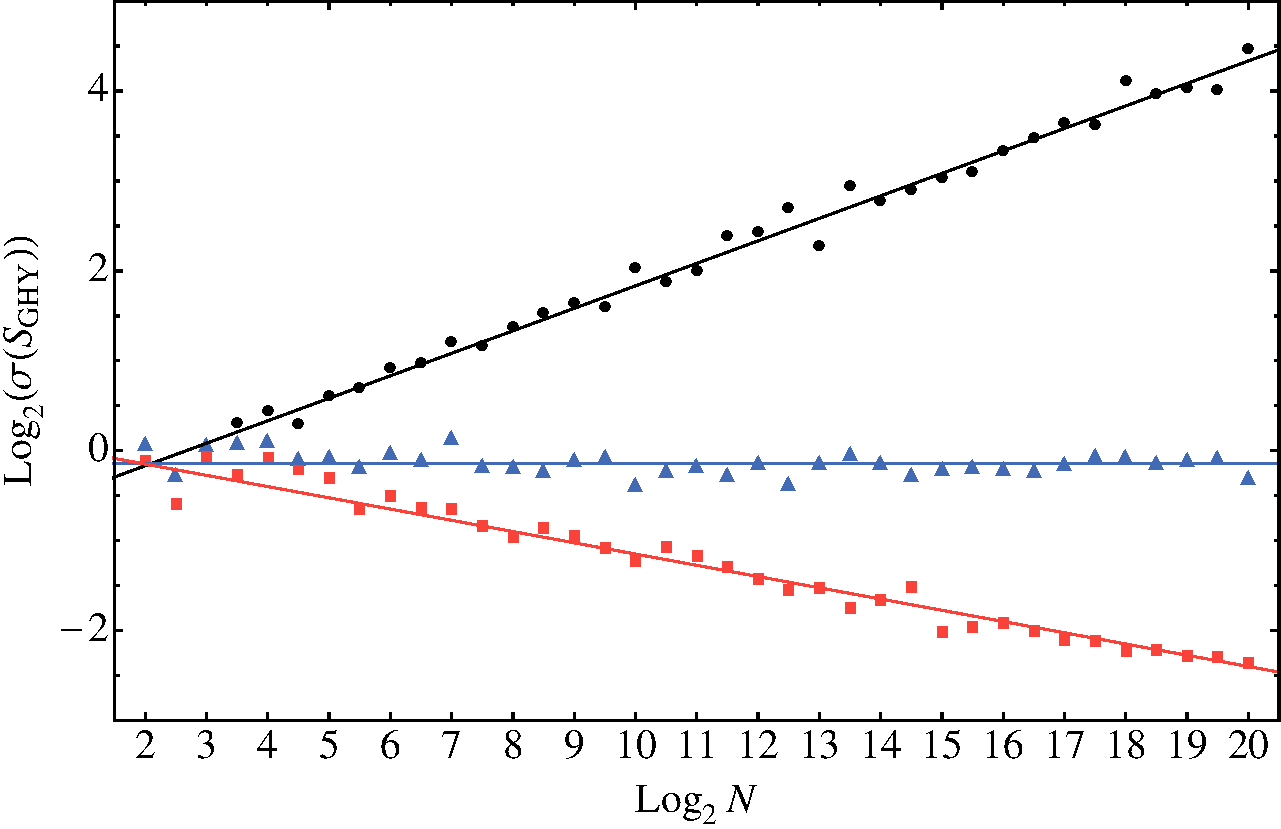
\includegraphics[scale=0.6]{GHY-fluctuation_plots}}
     \caption{A $\log-\log$ plot (base $2$) of the fluctuations in $S^{ (d)}_{GHY}$ for a flat ($K=0$) surface in $d=2,3$ and $4$-dimensional Minkowski space. Each data point represents the sample standard deviation in $S^{ (d)}_{GHY}$ on a sample of $R=100$ runs. Black dots, blue triangles and red squares correspond to the simulation results in $d=2,3$ and $4$ dimensions, respectively. The corresponding black, blue and red lines have gradients $\frac12$, $0$ and $-\frac18$ and best-fit intercepts of order $1$.}
     \label{fig:fluctuations}
\end{figure}

 
The simulations were carried out as follows. Denote the discreteness scale by $l$. Take a $d$-cube $[0,L]^d$ in $d$-dimensional Minkowski space with metric $ds^2=-dt^2+d{\mathbf x}^2$ and define the hypersurface $\Sigma: t=L/2$, which partitions the cube into two equal halves. Sprinkle at density $\rho=l^{-d}$ into the cube, which in any given run will place $N$ points inside the cube, where $N$ is the realisation of the Poisson random number $\textbf{N}$ with mean $\left\langle \textbf{N}\right\rangle = \rho V=  (L/l)^d$. Evaluate $S^{ (d)}_0=\rho^\frac{2-d}{d}c_d\left (2\Gamma\left (\frac{2}{d}\right)\right)^{-1} (\F{0} - \P{0})$ for $\Sigma$ by counting the minimal/maximal elements in the upper/lower half of the cube ($S^{ (d)}_0$, $\F{0}$, and $\P{0}$ of course being realisations of the random variables $\textbf{S}^{ (d)}_0$, $\BF{0}$, and $\BP{0}$), and repeat for $R$ runs. The value we expect for the mean (sum of all $S^{ (d)}_0$ values for each run divided by $R$) is zero in all cases, since the extrinsic curvature of the surface is zero.

In Figure~\ref{fig:fluctuations} we display the simulation results for $d=2,3,4$ spacetime dimensions, with $\left\langle\textbf{N}\right\rangle=\rho$ ranging up to $2^{20}\approx 1$ million, having set $V=L^d=1$. Each data point represents the fluctuations (the standard deviation) in a sample of $R=100$ runs. The solid lines have been obtained by fitting an arbitrary constant multiplier in the scaling law predicted by the argument above, $\gamma (d)\times \left\langle\textbf{N}\right\rangle^\frac{3-d}{2d}$, to the data sets. The best fit values are all of order $1$: $\gamma (2)=0.63$, $\gamma (3)=0.91$, and $\gamma (4)=1.07$.
There is clearly a good fit between the data and the scaling predicted by the heuristic argument. Although not visible on the plot, the data points were all consistent with zero mean as well.

As mentioned above, we have performed analogous simulations for other family members, such as $\mathbf S^{ (d)}_+$. This expression involves the terms $\BF{0}$ and $\BF{1}$, which means that heuristic arguments of the type given above are hampered by the fact that the two random variables whose difference is taken are not independent. However, the results for the scaling of the fluctuations turn out to be identical to those obtained in the first case.

\section{A Candidate Boundary Term for an Alexandrov Interval}
\newcommand{\vol}{\mathrm{vol}}

Until now our approach has been to reconstruct the  continuum GHY term  from the information in a causal set. 
The candidate described in the previous sections for a spatial boundary has a natural expression in a causal set  in  terms of its maximal and minimal elements. A suitable analog of a timelike boundary  term has been harder to  construct; there is no simple causal set  characterisation of such  a boundary. Indeed, it is difficult to give a causal set  characterisation of a spacetime region bounded by timelike surfaces. On the other hand, this is not true of causally defined spacetime regions since  past and future sets are defined naturally in  a causal set. An important example of such a region is the  Alexandrov interval which is used extensively  in calculations of causal set kinematics. In the continuum such a region is bounded by null hypersurfaces and their codimension-2 joints.  

Conversely in the continuum, while the GHY term  is well defined for both a space-like and time-like boundary  (including their codimension-2 joints)  it is an open question what the contribution from a null  boundary  is \cite{Gibbons_Hawking_Boundary, Harris}. Apart from some sketchy suggestions in the literature \cite{neiman} there is no rigourous construction of such a term; indeed the standard variational route for finding the boundary contribution to the action appears to fail for null boundaries. 

Given our ignorance in this matter,  we can ask if causal set theory  might  in fact guide us in the right direction.   Our starting point is the $d$-dimensional  Benincasa-Dowker Action \cite{Benincasa_Dowker:The_Scalar_Curvature_of_a_Causal_Set, Dowker_Glaser:dAlembertians_for_Causal_Sets}, $S_{BD}^{(d)}$, which is a function on a causal set constructed from the functions $N_i^{ (d)}$ which return the number of $i+1$-element inclusive intervals in the causal set, and the function $N$ which simply returns the number of causet elements. The Benincasa-Dowker action can be written as
\begin{equation}
8 \pi G {S_{BD}^{ (d)}}\left[\mathcal C\right] = -\alpha_d \rho^{\frac{2-d}{d}}\biggl ( N[\mathcal C]+ \frac{\beta_d}{ \alpha_d} \sum_{i=1}^{n_d-1}  C^{ (d)}_{i} N _i^{ (d)}[\mathcal C] \biggr) 
\label{bd} 
\end{equation}  
with   
\begin{equation}
\begin{aligned}
 \alpha_d =   
\begin{cases}
\displaystyle
-\frac1{\Gamma\left (1+\frac2d\right)}c_d ^{2/d} \;   &d \, \, \mathrm{odd} \\
\displaystyle
- \frac{2}{\Gamma\left (1+\frac2d\right)}c_d ^{2/d}  \;   &d \, \,  \mathrm{even} \\
\end{cases}
%\quad\text{and}\quad 
\end{aligned}
\end{equation}
and
\begin{equation}
\begin{aligned}
\beta_d =
\begin{cases}\displaystyle
\frac{d+1}{2^{d-1}\Gamma\left (1+\frac2d\right)} c_d^{2/d}   \;   &d\mathrm{ \, \, odd}\\ 
\displaystyle
\frac{\Gamma\left (\frac{d}{2}+2\right)\Gamma\left (\frac{d}{2}+1\right)}{\Gamma\left (\frac{2}{d}\right)\Gamma\left (d\right)}c_d^{2/d}  &  d\mathrm{ \, \,  even}\\ 
\end{cases} 
\end{aligned}
\end{equation}
and
\begin{equation} 
n_d = 
\begin{cases} 
\frac{d-1}{2} + 2  \quad & d\mathrm{ \, \, odd}\\ 
\frac{d}{2} + 2  \quad &d\mathrm{ \, \,  even,}\\ 
\end{cases} 
\end{equation} 
where  $2^{-d/2} c_d$ is the volume of a unit Alexandrov interval $I (x,y)$, i.e., one for which the proper time $\tau (x,y)=1$. 
%%{ {\bf \color{red} this is not correct! $c_d= \vol (S^{d-2}) \frac{ 2^{\frac{2-d}{2}}}{d (d-1)}$ and $\vol (S^{d-2})$ the volume of the homogeneous $d-2$ sphere}}.  
The coefficients $C_i^{ (d)}$ of the terms $N_i^{ (d)}$ in the sum are
\begin{equation}
\label{cid}
 C_i^{ (d)}= 
\begin{cases} 
\displaystyle\sum_{k=0}^{i-1} (-1)^k\binom{i-1}{k} \frac{\Gamma\left(\frac{d}2(k+1)+\frac32\right)}{\Gamma\left (\frac{d+3}{2}\right) \Gamma\left (1+\frac{d}2k\right)}  \quad  &d\mathrm{ \, \, odd}\\ 
\displaystyle\sum_{k=0}^{i-1} (-1)^k\binom{i-1}{k} \frac{\Gamma\left (\frac{d}2 (k+1)+2\right)}{\Gamma\left (\frac{d}2+2\right) \Gamma\left (1+\frac{d}2k\right)}  &d \mathrm{ \, \,  even.}\\ 
\end{cases} 
\end{equation} 
These coefficients can be expressed more compactly as hypergeometric functions 
\begin{equation}
C_i^{(d)}={}_{q+1}F_{q} (\{ a_1, \ldots, a_q, i-1\}, \{b_1, \ldots b_q \} |1)
\label{chyp} 
\end{equation} 
with $q=\frac{d+1}{2}$, $a_i=\frac{d+2i}{d}$, $b_i=\frac{2i}{d}$ for $d$ odd and $q=\frac{d}{2}$, $a_i=\frac{d+2i+2}{d}$, and $b_i=\frac{2i}{d}$  for $d$ even.  

As above we can define the random variable counterpart through a sprinkling, denoted by $\textbf{S}^{ (d)}_{BD}$. We can take the mean over sprinklings and the limit of $\rho\rightarrow\infty$. In this limit we find the mean is equal to $2 S_{EH}$ evaluated on the spacetime that we sprinkled into. This result has been proved only for certain cases.

If $S_{BD}^{ (d)}$ were precisely the discrete analog of twice the Einstein Hilbert action {\it without} any boundary contributions, then in flat spacetime  $S_{BD}^{ (d)}$ should  vanish. However, as shown explicitly in \cite{bbdtwo} this is not the case for Alexandrov intervals in $d=2$  flat spacetime. Indeed, there is a residual contribution that goes to a non-vanishing constant in the continuum limit $N\rightarrow \infty$.  When the action is evaluated in rectangular regions in the same spacetime or for Alexandrov intervals in  the flat trousers spacetime, this is no longer the case. Thus, it seems plausible that the $d=2$ BD action contains boundary information. Moreover, in the case of Alexandrov intervals the asymptotic value of the action is the same  irrespective of the interval size. While this might suggest a  topological origin, we will now show that it is a part of a more general  result for $d>2$ and  has a geometrical origin. Namely it corresponds to the volume  $\vol (S^{d-2})$ of the $S^{d-2}$ joint which is independent of the interval size {\it only} in $d=2$.

Consider an Alexandrov interval $I (p,q)=I^+ (p) \cap I^- (q)$ for two events $p,q$ in a causal spacetime.   While the  boundary of $I (p,q)$ may be quite complicated in general, some of these components must necessarily be null.  In flat spacetime, for example,  the boundary of $I (p,q)$ consists of the two events $p$ and $q$, the subsets $B^\pm$ of the  two null hypersurfaces $\partial J^+ (p)$ and $\partial J^- (q)$, and their intersection or ``joint''  $S^{d-2}=\partial J^+ (p) \cap \partial J^- (q)$ which is a codimension 2 sphere.  Evaluating the BD action in an Alexandrov interval in flat spacetime should therefore yield  only boundary dependent terms.  In flat spacetime the $S^{d-2}$ joint  has radius $\tau (p,q)/2$, and thus increases with the size of the Alexandrov interval ${\mathrm{vol}} (I (p,q)) = N/\rho$, where $N$ is the mean of the number of causal set elements sprinkled into $I (p,q)$ . In what follows we take the continuum limit $\rho, N \rightarrow \infty$ while keeping ${\mathrm{vol}} (I (p,q))$ fixed. \ss{It would be nice to have a fancy picture of an Alex. interval here..}  
%% If $p$ or $q$ were to be taken to time-like past or future infinity, this volume would go to infinity as expected.

In \cite{Glaser_Sumati:Locality_in_Causal_Set} a closed form expression was obtained for the mean value of the number of $i+1$ element inclusive intervals $N_i^{(d)}$ contained in an Alexandrov interval in $d$ dimensional flat spacetime 
\begin{equation} N_i^{ (d)}= \frac{\Gamma\left (d\right)^2 N^{i+2}}{\Gamma\left (i\right)} \sum_{k=0}^\infty \frac{ (-N)^k\,\Gamma\left (\frac{d}2 (k+i)+1\right)  \Gamma\left (\frac{d}2 (k+i+1)+1\right)}{ (k+i+2)  (k+i+1) \Gamma\left (k+1\right)\Gamma\left (\frac{d}2 (k+i) +d\right) \Gamma\left (\frac{d}2 (k+i+1)+d\right)},\nonumber
\end{equation} 
where $i \geq 1$.  We use this to expand the sum in (\ref{bd}) as a power series in $N$: $\sum_{i=1}^{n_d}C_i^{ (d)} N_i^{ (d)} = \sum_{j=1}^\infty A_j^{ (d)}  N^{j+1}$.  After a rearrangement and redefinition of indices we find that 
\begin{equation}
 A_j^{ (d)} = \Gamma\left (d\right)^2\frac{ (-1)^j}{ (j+1)!}\frac{\Gamma\left (\frac{d}{2} (j-1)+1\right)\Gamma\left (\frac{d}{2}j+1\right)}{\Gamma\left (\frac{d}{2} (j-1)+d\right) \Gamma\left (\frac{d}{2}j+d\right)}\sum_{i=1}^{D+2} (-1)^i \binom{j-1}{i-1}  C_i^{ (d)}, 
\end{equation} 
where $d=2D$ for $d$ even and $d=2D+1$ for $d$ odd.   
% Using the abbreviated form $C_i^d=\sum_{l=0}^{i-1} \binom{i-1}{l}A (d,l)$ where $A (d,l)$ is defined using \ref{cid} 
% we find that 
% \begin{equation}
% \sum_{i=1}^{D+2} (-1)^i \binom{j-1}{i-1}  C_i^d = (-1)^{j-1} A (d,j-1),  
% \end{equation}      
% where we have used the binomial identities  BLAH. Thus 
% \begin{equation}
%  \sum_{i=1}^{n_d} C_i^d N_i^{ (d)}= ( (d-1)!)^2 \sum_{j=1}^\infty (-1)^j B (d,j) \frac{\Gamma (\frac{d}{2}j+1)}{\Gamma (j+2)\Gamma (\frac{d}{2} (j-1)+d)\Gamma (\frac{d}{2}j+d)}N^{j+1}
% \label{thesum} 
% \end{equation} 
% where 
% \begin{equation} 
% B (d,j) = \left \{ 
% \begin{array}{ccc} 
% \frac{\Gamma (\frac{d}{2}j+3/2)}{\Gamma\left (\frac{d}{2}+3/2)}  &\quad & d \, \, odd, \\  \frac{\Gamma\left (\frac{d}{2}j+2\right)}{\Gamma\left (\frac{d}{2}+2\right)}  &\quad & d \, \, even.  \\ 
% \end{array} 
% \right
% \end{equation} 
This can be simplified to 
\begin{equation}
A_j^{(d)}=   \frac{\Gamma\left (d\right)^2 (-1)^{j+1}}{\Gamma\left (\frac{d}{2} (j + 1)\right) \Gamma\left (\frac{d}{2} (2 + j)\right) \Gamma\left (2 + j\right) } \gamma_j^{ (d)}
\label{simplercoefft} 
\end{equation} 
where 
\begin{equation} \gamma_j^{ (d)}= 
\begin{cases} 
\displaystyle\frac{\sqrt{\pi}}{2^{1+dj} }\frac{\Gamma\left (2+dj\right)}{\Gamma\left (\frac{d-1}{2}\right)}    \quad   & d \, \, \mathrm{odd} \\
\displaystyle\frac{\Gamma\left (1+\frac{d}{2}j\right)  \Gamma\left (2+\frac{d}{2}j\right) }{\Gamma\left (\frac{d}{2}\right)}  \quad  & d\mathrm{ \, \,  even.} \\
\end{cases} 
\end{equation} 
A further simplification then allows us to include the first term in the action (\ref{bd}) in the series expansion so that 
\begin{equation} 
8 \pi G S_{BD}^{ (d)}[\mathcal C] = -\alpha_d \rho^{\frac{2-d}{d}} \sum_{j=0}^\infty (-1)^j Q_j^{ (d)} N^{j+1} 
\end{equation}
where 
\begin{equation} 
Q_j^{ (d)}  = {\widetilde \gamma}_j^{\, (d)} \, \, \frac{\Gamma\left (d\right)\Gamma\left (\frac{d}{2}\right)}{\Gamma\left (\frac{d}{2} (1+j)\right) \Gamma\left (\frac{d}{2} (2+j)\right) \Gamma\left (2+j\right)}
\label{fullcoefft} \end{equation}
and
\begin{equation}
{\widetilde \gamma}_j^{\, (d)} = 
\begin{cases} 
2^{-dj}    \quad   &{d} \, \, \mathrm{odd} \\
\Gamma\left (1+\frac{d}{2}j\right) \Gamma\left (2+\frac{d}{2}j\right)   \quad   &d\mathrm{ \, \,  even.} \\
\end{cases} 
\end{equation} 
Taking our cues from the behaviour of $8 \pi G S_{BD}^{ (d)}[\mathcal C]$ for $d=2,3$ in the  $N \rightarrow \infty$ limit,  we will consider the ratio
\begin{equation} 
\frac{ 8 \pi G S_{BD}^{ (d)}[\mathcal C]}{\vol (S^{d-2})} = \frac{b}{d (d-1) \Gamma\left (1+\frac2d\right) N^{\frac{d-2}{d}}} \left ( N + \frac{\beta_d}{\alpha_d} \sum_{i=1}^{n_d} C_i^{ (d)} N_i^{ (d)} \right)  
\label{ratio} 
\end{equation} 
where $b=1$ for $d$ odd and $b=2$ for $d$ even.
Using this simplification an explicit calculation in Mathematica\footnote{The above simplifications greatly aid the Mathematica calculation and allow us to extend it to higher $d$.}  for $d=2, \ldots, 16$ gives 
\begin{equation} 
\lim_{N \rightarrow \infty} \frac{ 8 \pi G S_{BD}^d (C)}{\vol (S^{d-2})} = 1,  
\label{result} 
\end{equation} 

Since each $N_i^{ (d)}$  can be expressed as a hypergeometric function \cite{Glaser_Sumati:Locality_in_Causal_Set} it  might seem possible to evaluate (\ref{ratio}) analytically term by term using a large $N$ expansion.  In \cite{Glaser_Sumati:Locality_in_Causal_Set} the asymptotic form of $N_i^{ (d)}$ was explicitly calculated, and for $d>2$, the leading order was shown to  $\sim  N^{2-\frac{2}{d}}$. This provides us a good consistency check for our result (\ref{result}) since this would mean that the leading order contributions from the $N_i^{ (d)}$ cancel in the action. This is indeed explicitly seen to be the case, again for $d=3, \ldots 16$. Similarly for $d=2$ where the leading order contribution is $\sim  N \log N$.  Indeed, in all cases the next to leading order terms given in \cite{Glaser_Sumati:Locality_in_Causal_Set} also do not have the requisite $ \sim N^{\frac{d-2}{d}}$ dependence required by (\ref{result}); in this case, the explicit coefficients have not been calculated  to be able   check for  a vanishing contribution to (\ref{result}).  This suggests that  we cannot rely   on the the asymptotic form of the individual terms  in the sum, and would need to look elsewhere to find an analytic proof for general $d$. While it may be possible to use the simplification (\ref{fullcoefft})  to obtain a closed form expression for the action for general $d$, it suffices for our purposes that (\ref{result}) has been explicitly checked in $2\leq d \leq 16$ dimensions.  

The result we have obtained is for flat spacetime. One may speculate that the presence of curvature will not modify the essence of this result,  i.e., that the BD action for an Alexandrov interval  will include boundary contributions from the  $S^{d-2}$ at the joint, at least  when the boundary components  are of the same type as in flat spacetime.   What will differ of course is the fact that the principal radii of the $S^{d-2}$ will in general vary from point to point, hence complicating the relationship between the $d$-volume of the interval and the $ (d-2)$-volume of $S^{d-2}$. In  \cite{Khetrapal_Sumati:Causal_Diamond_Volume} it was shown that in an RNC up to first order corrections the intrinsic boundary geometry of the Alexandrov interval is still flat. This would allow a simpler relation between $\vol (S^{d-2})$ and $N$, making it possible to do an RNC version of this  calculation. 

The fact that the BD action does not vanish in flat spacetime suggests  that this action  does not only contain  information about the bulk Einstein Hilbert action but also extra boundary information.  One might be tempted to speculate further that this action contains {\it all}  possible boundary or GHY terms suggesting that the null boundary GHY contribution for an Alexandrov interval in any spacetime always vanishes. Moreover, it is only the spatial $S^{d-2}$ joint  which gives  a non-vanishing contribution $\vol (S^{d-2})$.  Interestingly, this is precisely what \cite{neiman} claims is the GHY term for an Alexandrov interval. 

\newpage




\bibliographystyle{jhep}

\bibliography{references}

\end{document}


%%
JHEPPUB:

\title{Gibbons-Hawking-York Boundary Term in Causal Sets}
 \author[a]{M. Buck}
 \author[a,b]{\!, F. Dowker}
 \author[a]{and I. Jubb\,}
\affiliation[a]{Theoretical Physics Group, Blackett Laboratory, Imperial College, London, SW7 2AZ, U.K.}
\affiliation[b]{Institute for Quantum Computing, University of Waterloggedo, ON, N2L 2Y5, Canada}

\abstract{ 
We show some stuff.
}

\begin{document}

\maketitle

\pagebreak

\noindent NOTES:\\
1. define s as the RV, not as its mean

\section{Introduction}




%%IOPART

\begin{document}

\title{Gibbons-Hawking-York Boundary Term in Causal Sets}

\author{Michel Buck Fay Dowker, Ian Jubb}
\address{Blackett Laboratory, Imperial College, London, SW7 2AZ, U.K.}

\begin{abstract}

We show some stuff.

\end{abstract}
%\pacs{03.67.-a, 03.65.Ta, 03.70.+k}

\maketitle
\section{Introduction}
%%

